  %\begin{figure}[H]
\begin{wrapfigure}[10]{R}{0.6\textwidth}
\vspace{-35pt}
  \begin{center}
  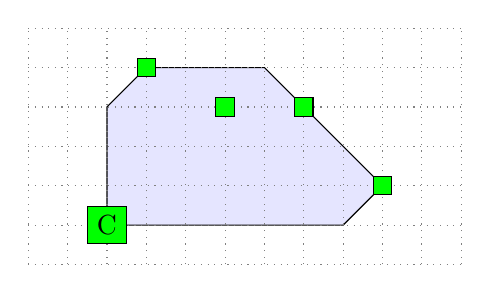
\begin{tikzpicture}[scale=0.5]
    %\draw[fill=red!10] (0,6) -- (0,0) -- (2,4) -- cycle;
    \draw[fill=blue!10] (2,1) -- (2,4) -- (3,5) -- (6,5) -- (9,2) -- (8,1) -- cycle;
    %\draw[fill=yellow!10] (3,6) -- (3,5) -- (6,1) -- (6,2) 
      -- cycle;
    %\draw[fill=green!10] (7,6) -- (12,6) -- (10,4) -- (5,4) 
      -- cycle;
    %\draw[fill=orange!10] (12,4) -- (11,0) -- (12,0) -- cycle;
    \draw[color=gray, style=dotted] (0,0) 
      grid[xstep=1cm, ystep=1cm] (11cm,6cm);
  	\node at (2,1) [draw,fill=green] {C};
  	%\node at (1.5,0.5) [draw=none]	 {C};
  	%\node at (9.5,1.5) [draw=none]	 {D};
  	\node at (3,5) [draw,fill=green] {};
  	\node at (9,2) [draw,fill=green] {};
  	\node at (7,4) [draw,fill=green] {};
  	\node at (5,4) [draw,fill=green] {};
  \end{tikzpicture}
  \caption{The octagonal hull of green points. The green point marked with the letter $C$ is a {\em corner} of the octagon hull.}
  % Clearly intersection with lines will be segments of lines. }
  \label{expotential}
  \end{center}
%  \end{figure}
\end{wrapfigure}